\documentclass[aspectratio=169, xcolor=dvipsnames]{beamer}
\hypersetup{pdfpagemode=FullScreen}
\beamertemplatenavigationsymbolsempty
\setbeamertemplate{caption}{\raggedright\insertcaption\par}
\usepackage[utf8]{inputenc}
\usepackage[spanish]{babel}
\usepackage{siunitx}
\usepackage{graphicx}
\usepackage{xcolor}
\usepackage{amsmath}
\usepackage{esint}
\usepackage{biblatex}
\usepackage{multicol}
\setlength\columnsep{20pt}
\usepackage{listings}

\definecolor{mygreen}{rgb}{0,0.6,0}
\lstdefinestyle{mystyle}{
    commentstyle=\color{mygreen},
    keywordstyle=\color{blue},
}
\lstset{style=mystyle}

\definecolor{myblue}{rgb}{0.29, 0.5, 0.94}

\title{Aplicaciones de Sistemas Embebidos con Doble Núcleo}
\subtitle{Sistemas Embebidos en Lenguaje C}
\author[Fabrizio Carlassara - Laboratorio de Sistemas Embebidos]{
\includegraphics[scale=0.15]{resources/images/utn_logo.png}}
\institute{UTN FRA\\Departamento de Ingeniería Electrónica\\Laboratorio de Sistemas Embebidos}
\date[]{\today} 
\usetheme{Warsaw}
\usecolortheme[named=myblue]{structure}
\setbeamertemplate{headline}{}

\begin{document}

\frame{\titlepage}
\begin{frame}{Sistemas Embebidos en Lenguaje C}{Índice}
\begin{multicols}{3}
\tableofcontents
\end{multicols}
\end{frame}

\section{Por qué C?}
\begin{frame}{Sistemas Embebidos en Lenguaje C}{Por qué C?}
\begin{columns}
    \begin{column}{0.75\textwidth}
    \begin{itemize}
        \item Lenguaje compilado.
        \item Determinista.
        \item Acceso directo a memoria, periféricos y hardware.
        \item Rápido y fácilmente optimizable.
        \item Mucho soporte en bibliotecas.
        \item Fácilmente portable a otros microcontroladores.
        \item Sintáxis sencilla.
        \item Soporte en la totalidad de microcontroladores.
        \item Permite un uso eficiente de memoria volátil y no volátil.
    \end{itemize}
    \end{column}
    \begin{column}{0.25\textwidth}
        \begin{figure}
            \centering
            
\includegraphics[width=0.5\linewidth]{resources/images/c_logo.png}
        \end{figure}
    \end{column}
\end{columns}
\end{frame}

\section{Tipos de datos}
\subsection{Enteros}
\subsubsection{Tipos}
\begin{frame}{Sistemas Embebidos en Lenguaje C}{Enteros - Tipos}
% \noindent\rule{\textwidth}{0.75pt}
\begin{columns}
    \begin{column}{0.5\textwidth}
    \begin{itemize}
        \item Existen en variantes de 8, 16, 32 y 64 bits.
        \item Preceder la declaración del tipo de entero con la palabra \lstinline[language=c]{unsigned} hace que toda la capacidad de la variable sea para numeros positivos.
        \item Pueden representar $2^n$ números, siendo n la cantidad de bits.
    \end{itemize}
    \end{column}
    \begin{column}{0.5\textwidth}
        \lstinputlisting[language=c]{resources/listings/data_type_int.c}
    \end{column}
\end{columns}
\end{frame}

\subsubsection{Estandarización}
\begin{frame}{Sistemas Embebidos en Lenguaje C}{Enteros - Estandarización}
    Podemos usar la biblioteca \textcolor{myblue}{stdint.h} que generalmente tenemos incluida para poder usar nombres más estándares para estos tipos de datos enteros.
    \lstinputlisting[language=c]{resources/listings/data_type_stdint.c}
    % \noindent\rule{\textwidth}{0.75pt}
\end{frame}

\subsection{Flotantes}
\subsubsection{Tipos}
\begin{frame}{Sistemas Embebidos en Lenguaje C}{Flotantes - Tipos}
\begin{columns}
    \begin{column}{0.5\textwidth}
        \begin{itemize}
            \item Sirven para representar números con decimales.
            \item El tipo \textcolor{myblue}{float} es una variante de 32 bits con 7 decimales de precisión.
            \item El tipo \textcolor{myblue}{double} es una variante de 64 bits con 15 decimales de precisión.
            \item Siguen el estándar de punto flotante IEEE 754.
            \item El tipo \textcolor{myblue}{float} tiene un rango de valores de $3.4 x 10^{-38}$ a $3.4 x 10^{38}$.
            \item El tipo \textcolor{myblue}{double} tiene un rango de valores de $1.7 x 10^{-308}$ a $1.7 x 10^{308}$.
        \end{itemize}
    \end{column}
    \begin{column}{0.5\textwidth}
        \lstinputlisting[language=c]{resources/listings/data_type_float.c}
    \end{column}
\end{columns}
\end{frame}

\subsubsection{Representación IEEE 754}
\begin{frame}{Sistemas Embebidos en Lenguaje C}{Flotantes - Representación IEEE 754}
\begin{columns}
    \begin{column}{0.5\textwidth}
    \begin{figure}
        \centering
        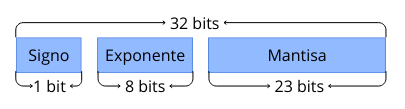
\includegraphics[width=0.9\linewidth]{resources/images/float_ieee_754.png}
        \caption{Float en IEEE 754}
    \end{figure}
    \begin{figure}
        \centering
        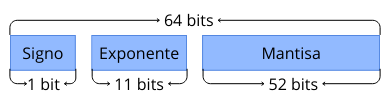
\includegraphics[width=0.9\linewidth]{resources/images/double_ieee_754.png}
        \caption{Double en IEEE 754}
    \end{figure}    
    \end{column}
    \begin{column}{0.5\textwidth}
    \begin{itemize}
        \item Bit más significativo para el signo (0 positivo y 1 negativo).
        \item Los siguientes 8/11 bits se usan para almacenar el exponente con un offset ya que no se almacena directamente un exponente negativo.
        \item Los últimos 23/52 bits se usan para la mantisa, es decir, el número normalizado en notación científica.
    \end{itemize}
    \end{column}
\end{columns}
\end{frame}

\subsection{Arrays}
\begin{frame}{Sistemas Embebidos en Lenguaje C}{Arrays}
\begin{columns}
    \begin{column}{0.5\textwidth}
        \begin{itemize}
            \item Es un conjunto de elementos del mismo tipo de dato.
            \item Un array de $n$ elementos de $b$ bytes ocupará en la memoria $n \times b$ bytes.
            \item La primera posición del array es la 0.
            \item Un array de $n$ elementos tiene posiciones desde 0 hasta $n - 1$.
        \end{itemize}
    \end{column}
    \begin{column}{0.5\textwidth}
        \lstinputlisting[language=c]{resources/listings/data_type_array.c}
    \end{column}
\end{columns}
\end{frame}

\subsection{Punteros}
\subsubsection{Características}
\begin{frame}{Sistemas Embebidos en Lenguaje C}{Punteros - Características}
\begin{itemize}
    \item Guardan la dirección de una variable.
    \item Con el operador \textbf{\&} se puede ver la dirección de una variable, incluso un puntero.
    \item Con el operador \textbf{*} se puede ver el valor en la dirección que almacena el puntero.
    \item Se usan en pasajes por referencia.
    \item Permiten ver el valor de la dirección que guardan y modificarlo.
    \item Los arrays pueden usarse como punteros.
\end{itemize}
\end{frame}

\subsubsection{Operadores especiales}
\begin{frame}{Sistemas Embebidos en Lenguaje C}{Punteros - Operadores especiales}
\begin{columns}
    \begin{column}{0.5\textwidth}
    \lstinputlisting[language=c]{resources/listings/data_type_pointer.c}
    \end{column}
    \begin{column}{0.5\textwidth}
    \begin{figure}
        \centering
        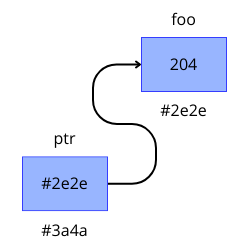
\includegraphics[width=0.75\linewidth]{resources/images/punteros.png}
    \end{figure}
    \end{column}
\end{columns}
\end{frame}

\subsection{Estructuras}
\subsubsection{Declaración y typedef}
\begin{frame}{Sistemas Embebidos en Lenguaje C}{Estructuras - Declaración y typedef}
\begin{columns}
    \begin{column}{0.5\textwidth}
        \begin{itemize}
            \item Es un conjunto de elementos pero no necesariamente del mismo tipo de dato.
            \item Cada elemento que la compone se denomina campo y tiene un nombre y tipo de dato asociado.
            \item Usando la palabra \textcolor{myblue}{typedef} podemos definir a una estructura como un nuevo tipo de dato.
        \end{itemize}
    \end{column}
    \begin{column}{0.5\textwidth}
        \lstinputlisting[language=c]{resources/listings/data_type_struct_1.c}
    \end{column}
\end{columns}
\end{frame}

\subsubsection{Asignación y campos}
\begin{frame}{Sistemas Embebidos en Lenguaje C}{Estructuras - Asignación y campos}
\begin{columns}
    \begin{column}{0.5\textwidth}
        \begin{itemize}
            \item Para acceder a un campo, se usa el operador \textbf{.} entre el nombre de la variable y el nombre del campo.
            \item Con los campos, se ordena mejor la información de un conjunto de datos.
        \end{itemize}
    \end{column}
    \begin{column}{0.5\textwidth}
        \lstinputlisting[language=c]{resources/listings/data_type_struct_2.c}
    \end{column}
\end{columns}
\end{frame}

\subsubsection{Punteros}
\begin{frame}{Sistemas Embebidos en Lenguaje C}{Estructuras - Punteros}
\begin{columns}
    \begin{column}{0.5\textwidth}
        \lstinputlisting[language=c]{resources/listings/data_type_struct_3.c}
    \end{column}
    \begin{column}{0.5\textwidth}
        \begin{itemize}
            \item Es posible crear punteros a estructuras que se definan.
            \item Cuando se maneja un puntero a estructura, para acceder a un campo se usa el operador \textbf{$->$}.
        \end{itemize}
    \end{column}
\end{columns}
\end{frame}

\section{Condicionales}
\subsection{Generalidades}
\begin{frame}{Sistemas Embebidos en Lenguaje C}{Condicionales - Generalidades}
\begin{itemize}
    \item La condición que se evalúa, se escribe entre paréntesis.
    \item Sólo importa si la condición o valor en el paréntesis termina siendo algo interpretable como verdadero o falso.
    \item Se pueden usar los operadores \textbf{$==$}, \textbf{$>$}, \textbf{$>=$}, \textbf{$<$}, \textbf{$<=$} o \textbf{$!=$} para comparar expresiones.
    \item Para concatenar múltiples condiciones, se usa el operador $||$ (OR) o el operador \&\& (AND).
    \item En el caso de los switch case, los casos se evalúan sólo por igualdad.
\end{itemize}
\end{frame}

\subsection{if}
\begin{frame}{Sistemas Embebidos en Lenguaje C}{Condicionales - if}
\begin{columns}
    \begin{column}{0.5\textwidth}
    \begin{figure}
        \centering
        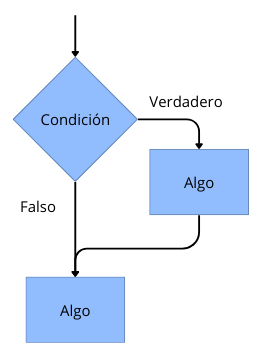
\includegraphics[width=0.6\linewidth]{resources/images/if.png}
    \end{figure}
    \end{column}
    \begin{column}{0.5\textwidth}
    \lstinputlisting[language=c]{resources/listings/if.c}
    \end{column}
\end{columns}
\end{frame}

\subsection{if ... else}
\begin{frame}{Sistemas Embebidos en Lenguaje C}{Condicionales - if ... else}
\begin{columns}
    \begin{column}{0.5\textwidth}
    \begin{figure}
        \centering
        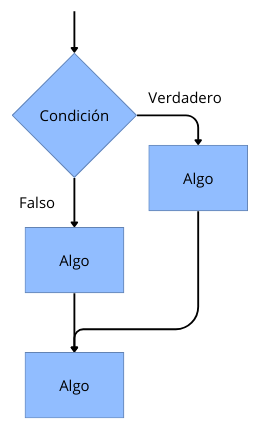
\includegraphics[width=0.5\linewidth]{resources/images/if_else.png}
    \end{figure}
    \end{column}
    \begin{column}{0.5\textwidth}
        \lstinputlisting[language=c]{resources/listings/if_else.c}
    \end{column}
\end{columns}
\end{frame}

\subsection{if ... else if ... else}
\begin{frame}{Sistemas Embebidos en Lenguaje C}{Condicionales - if ... else if ... else}
\begin{columns}
    \begin{column}{0.5\textwidth}
        \lstinputlisting[language=c]{resources/listings/if_else_if_else.c}
    \end{column}
    \begin{column}{0.5\textwidth}
        \begin{figure}
            \centering
            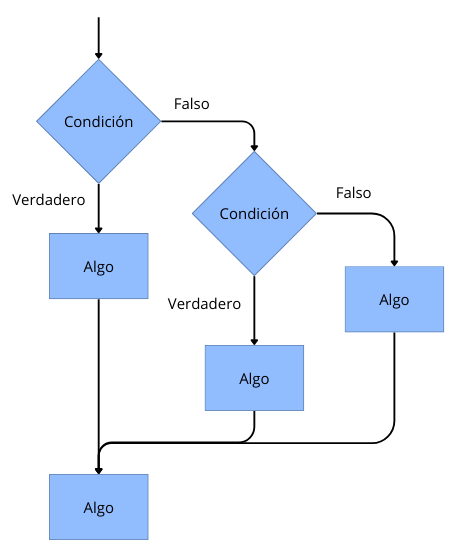
\includegraphics[width=0.75\linewidth]{resources/images/if_else_if_else.png}
        \end{figure}
    \end{column}
\end{columns}
\end{frame}

\subsection{switch ... case}
\begin{frame}{Sistemas Embebidos en Lenguaje C}{Condicionales - switch ... case}
\begin{columns}
    \begin{column}{0.6\textwidth}
        \begin{figure}
            \centering
            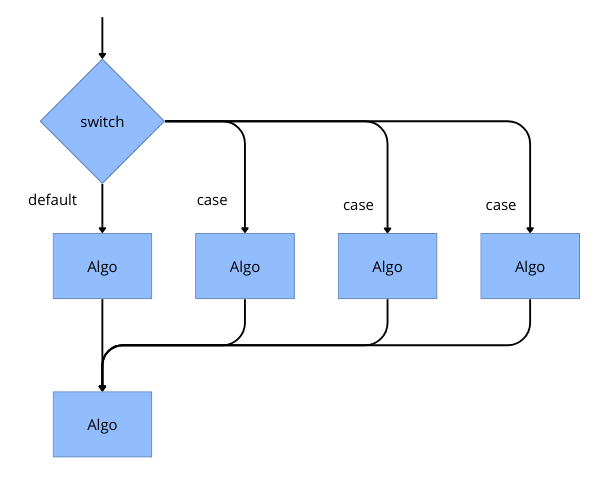
\includegraphics[width=0.8\linewidth]{resources/images/switch_case.png}
        \end{figure}
    \end{column}
    \begin{column}{0.4\textwidth}
        \lstinputlisting[language=c]{resources/listings/switch_case.c}
    \end{column}
\end{columns}
\end{frame}

\section{Bucles}
\subsection{while}
\begin{frame}{Sistemas Embebidos en Lenguaje C}{Bucles - while}
\begin{columns}
    \begin{column}{0.5\textwidth}
    \begin{itemize}
        \item Repiten el código expresado en las llaves mientras que la condición sea verdadera.
        \item La condición se evalúa antes de entrar al bucle, si es falsa, no se ejecuta ninguna iteración.
        \item La condición luego se evalúa al comenzar cada nueva iteración.
    \end{itemize}
    \end{column}
    \begin{column}{0.5\textwidth}
    \lstinputlisting[language=c]{resources/listings/while.c}
    \end{column}
\end{columns}
\end{frame}

\subsection{do ... while}
\begin{frame}{Sistemas Embebidos en Lenguaje C}{Bucles - do ... while}
\begin{columns}
    \begin{column}{0.5\textwidth}
    \lstinputlisting[language=c]{resources/listings/do_while.c}
    \end{column}
    \begin{column}{0.5\textwidth}
    \begin{itemize}
        \item La condición para iterar se escribe el final.
        \item A diferencia del while tradicional, la condición se evalúa al final de cada iteración.
        \item Son útiles donde por lo menos debe asegurarse una iteración.
    \end{itemize}
    \end{column}
\end{columns}
\end{frame}

\subsection{for}
\begin{frame}{Sistemas Embebidos en Lenguaje C}{Bucles - for}
\begin{columns}
    \begin{column}{0.5\textwidth}
    \begin{itemize}
        \item Se puede asignar un valor inicial a una variable (condición inicial) en el primer argumento del bucle.
        \item La condición para iterar se escribe en el segundo argumento.
        \item En cada iteración, se puede incrementar el valor de una variable. El incremento se describe en el tercer argumento.
        \item El incremento puede ser positivo o negativo.
    \end{itemize}
    \end{column}
    \begin{column}{0.5\textwidth}
        \lstinputlisting[language=c]{resources/listings/for.c}
    \end{column}
\end{columns}
\end{frame}

\section{Funciones}
\subsection{Definición}
\begin{frame}{Sistemas Embebidos en Lenguaje C}{Funciones - Definición}
\begin{itemize}
    \item Ayudan a encapsular y abstraer código.
    \item Son un bloque de código con nombre, valores de entraday  valor de salida que se puede invocar cuando queramos.
    \item Pueden tener múltiples valores de entrada pero solo uno de salida.
    \item Si no devuelve o recibe valores, se define con la palabra \textcolor{myblue}{void}.
    \item Normalmente, se usa un prototipo, es decir, un descriptor de la función, antes de invocarla.
\end{itemize}
\begin{figure}
    \centering
    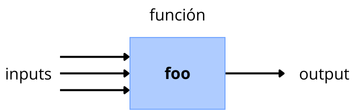
\includegraphics[width=0.5\linewidth]{resources/images/funciones.png}
\end{figure}
\end{frame}

\subsection{Parámetros}
\begin{frame}{Sistemas Embebidos en Lenguaje C}{Funciones - Parámetros}
\begin{columns}
    \begin{column}{0.5\textwidth}
    \begin{itemize}
        \item Son variables que recibe la función.
        \item Pueden usarse para operar dentro de la función.
        \item Se guardan en el stack.
        \item No existe límite a cuantos parámetros puede tener una función.
    \end{itemize}
    \lstinputlisting[language=c]{resources/listings/funciones_0.c}
    \end{column}
    \begin{column}{0.5\textwidth}
    \lstinputlisting[language=c]{resources/listings/funciones_1.c}
    \end{column}
\end{columns}
\end{frame}

\subsection{Retorno}
\begin{frame}{Sistemas Embebidos en Lenguaje C}{Funciones - Retorno}
\begin{columns}
    \begin{column}{0.5\textwidth}
    \lstinputlisting[language=c]{resources/listings/funciones_2.c}
    \end{column}
    \begin{column}{0.5\textwidth}
    \begin{itemize}
        \item El valor de retorno puede ser solo uno.
        \item La palabra \textcolor{myblue}{return} se usa para describir que valor o variable de la función se desea retornar.
        \item Al retornar, se termina la ejecución de la función.
        \item El retorno de una variable es la única forma de obtener algún valor que fue usado localmente en la función.
        \item Es posible guardar el retorno de una función en otra variable.
    \end{itemize}
    \end{column}
\end{columns}
\end{frame}

\section{Referencias}
\begin{frame}{Sistemas Embebidos en Lenguaje C}{Referencias}
    Algunos recursos útiles
    \noindent\rule{\textwidth}{0.75pt}
    \begin{multicols}{2}
    \begin{itemize}
        \item \href{https://www.h-schmidt.net/FloatConverter/IEEE754.html}{IEEE-754 Floating Point Converter}
        \item \href{https://vanhunteradams.com/FixedPoint/FixedPoint.html}{Aritmética de punto fijo}
        \item \href{https://www.geeksforgeeks.org/pass-by-reference-in-c/}{Pasaje por referencia}
        \item \href{https://www.geeksforgeeks.org/pointer-arithmetics-in-c-with-examples/}{Aritmética de punteros}
        \item \href{https://www.geeksforgeeks.org/structures-c/}{Estructuras}
        \item \href{https://unstop.com/blog/conditional-if-else-statements-in-c}{Condicionales}
        \item \href{https://www.geeksforgeeks.org/c-loops/}{Bucles}
        \item \href{https://www.geeksforgeeks.org/c-function-argument-return-values/}{Argumentos y retorno}
        \item \href{https://www.shiksha.com/online-courses/articles/difference-between-argument-and-parameter-blogId-147937}{Argumentos vs Parámetros}
    \end{itemize}
    \end{multicols}
\end{frame}

\end{document}
